\documentclass[border=3pt,tikz]{standalone}
\usepackage[utf8]{vietnam}
\usetikzlibrary{calc,angles,intersections,shapes.geometric,arrows,decorations.markings,arrows.meta,patterns.meta,patterns}
\usepackage{tikz-3dplot,pgfplots}
\pgfplotsset{compat=1.15}
\usepgfplotslibrary{polar}
\usepackage{amsmath}
\begin{document}
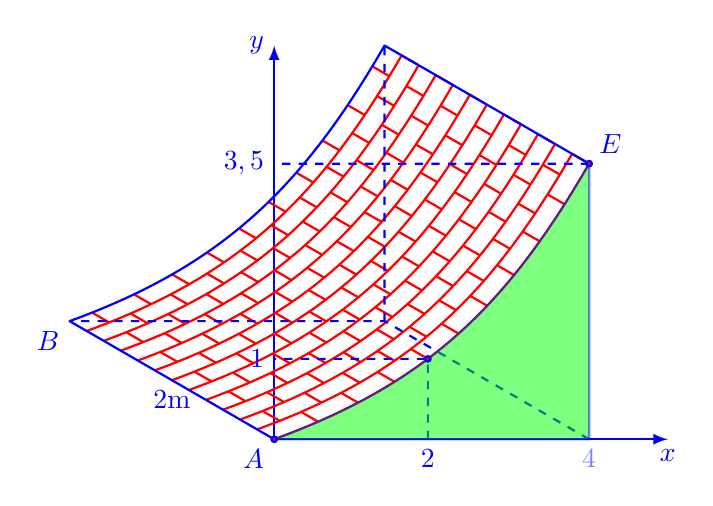
\begin{tikzpicture}[blue,thick, line join=round]
	\draw[latex-latex] (0,5)node[left]{$y$}|-(5,0)node[below]{$x$};
	%Vẽ gạch cong
	\foreach \x in {0,.5,...,2.5}{
		\begin{scope}[shift={(150:\x)}]
			\draw[red] (0,0) to[out=20,in=-120]
			coordinate[pos=.1](X1)
			coordinate[pos=.2](X2)
			coordinate[pos=.3](X3)
			coordinate[pos=.4](X4)
			coordinate[pos=.5](X5)
			coordinate[pos=.6](X6)
			coordinate[pos=.7](X7)
			coordinate[pos=.8](X8)
			coordinate[pos=.9](X9)
			coordinate[pos=1](X10)
			++(4,3.5);
			\draw[red] (150:.25) to[out=20,in=-120]
			coordinate[pos=.05](Y1)
			coordinate[pos=.15](Y2)
			coordinate[pos=.25](Y3)
			coordinate[pos=.35](Y4)
			coordinate[pos=.45](Y5)
			coordinate[pos=.55](Y6)
			coordinate[pos=.65](Y7)
			coordinate[pos=.75](Y8)
			coordinate[pos=.85](Y9)
			coordinate[pos=.95](Y10)
			++(4,3.5);
			\foreach \i in {1,...,10}\draw[red] (X\i)--++(150:.25) (Y\i)--++(150:.25);
		\end{scope}
	}
	%======
	\path (0,0)node[below left]{$A$}to[out=20,in=-120]coordinate[pos=.4](A)(4,3.5)node[above right]{$E$};
	\draw[dashed]($(0,0)!(A)!(4,0)$) node[below]{$2$}-- (A)--($(0,0)!(A)!(0,4)$)node[left]{$1$} (4,0)--++(150:3)--++(-4,0) (4,3.5)--(0,3.5)node[left]{$3,5$} ($(4,0)+(150:3)$)--++(0,3.5);
	\draw[fill=green,opacity=.5] (0,0)to[out=20,in=-120](4,3.5)--(4,0)node[below]{$4$}--cycle;
	\draw (0,0)--++(150:3)node[below left]{$B$}node[midway,below]{$2$m} to[out=20,in=-120]++(4,3.5)--(4,3.5);
	\draw[fill=red](0,0) circle (1pt) (4,3.5) circle (1pt) (A)circle (1pt);
\end{tikzpicture}
\end{document}